\section{Concurrency: Spin Locks and Bags}
% invariants and ghost state
\subsection{Later and persistent modalities}
\begin{itemize}
  \item The $\later$ modality expresses that a property is only supposed to hold later, after a reduction step has taken place
	\item The set of Iris proportions is not just a set of resources
  \begin{itemize}
  	\item An iris proposition $P$ is closer to being a set of pairs $(k,r)$ where $k$ is a natural number and $r$ a reource
    \item $k$ can be thought of as a step-index i.e. a natural number which expresses for how many reduction steps we know that $r$ is in $P$ 
    \item If $(k,r) \in P$ and $m \leq k$ then also $(m,r) \in P$ 
    \item The step-indices are used to interpret $\later$
    \[
      \later P=\{(m+1, r) \mid (m, r) \in P\} \cup\{(0, r) \mid r \in \mathcal{R}\}
    \]
    \item ``later'' means that the index number is smaller 
    \begin{itemize}
    	\item There are fewer reductions steps left after some reduction steps has been taken
    \end{itemize}
  \end{itemize}
  \item The persistent modality $\square$ is defined as follows
  \[
    \square P=\left\{r \in \mathcal{R} | \exists s, r^{\prime}, s \in P \wedge s=s \cdot s \wedge r=s \cdot r^{\prime}\right\}
  \]
  \begin{itemize}
  	\item $\square P$ is the upwards-closure of the set of duplicable resources in $P$
    \item Persistent predicates are those predicates that do not assert exclusive owner, over resources
    \item It only expresses ``knowledge'' and now exclusive ownership
    \item Persistent predicates $P$ are duplicable: $P \dashv\vdash P * P$
  \end{itemize}
  % TODO persistent rule for moving 
  \item There are two kinds of primitive persistent propositions 
  \[
    t =_\tau t' \dashv \vdash \square (t =_\tau t') \quad \{P\} e \{\Phi\} \dashv \vdash \square \{P\} e \{\Phi\}
  \]
  \item The rule \texttt{HT-PERSISTENTLY} can be used to move persistent propositions in and out of preconditions
  \[
  \begin{prooftree} 
    \hypo{\square Q \land S \vdash \{P\}\; e \; \{v.R\}}
    \infer[double]1{S \vdash \{P \land \square Q\}\; e \; \{v.R\}} 
  \end{prooftree}
  \]
\end{itemize}

\subsection{Proof rules}
\begin{itemize}
	\item $e_1 \mid \mid e_2$ runs $e_1$ and $e_2$ is parallel, waits until both finish, and then returns a pair consisting of the values to which $e_1$ and $e_2$ evaluated 
  \begin{itemize}
  	\item It is definable using fork
  \end{itemize}
  \item The following rule \texttt{HT-PAR}
  \[
  \begin{prooftree} 
    \hypo{S \vdash \{P_1\}e_1 \{v.Q_1\}}
    \hypo{S \vdash \{P_2\}e_2 \{v.Q_2\}} 
    \infer2{S \vdash \{P_1 * P_2\} e_1 \mid \mid e_2 \{v. \exists v_1v_2.v = (v_1,v_2) * Q_1[v_1/v] * Q_2[v_2/v]\}} 
  \end{prooftree}
  \]
  states that one can run $e_1$ and $e_2$ in parallel and if they have \textbf{disjoint} footprints and then verify the two components seperately 
  \begin{itemize}
    \item It is referred to as the \textbf{disjoint concurrency rule}
    \item Each thread is reasoned about in isolation (\textbf{thread-local reasoning}) 
  	\item Important since it is not possible to reason about all possible interleavings of threads since there are too many
  \end{itemize}
  % HT-CAS construct and rule 
  \item The following rule \texttt{HT-CAS}
  \[
  \begin{prooftree} 
    \infer0{\{\later \ell \hookrightarrow v\} \text{cas}(\ell,v_1,v_2)\{u.(u = \true * v = v_1 * \ell \hookrightarrow v_2) \lor (u = \false * v \neq v_1 * \ell \hookrightarrow v)\}} 
  \end{prooftree}
  \]
  is used for the general case of the cas primitive. 
  \begin{itemize}
    \item The derived rules \texttt{HT-CAS-SUCC}
    \[
    \begin{prooftree} 
      \infer0{\{\later \ell \hookrightarrow v_1\} \text{cas}(\ell,v_1,v_2)\{u.u = \true * v = v_1 * \ell \hookrightarrow v_2\}} 
    \end{prooftree}
    \]
    and \texttt{HT-CAS-FAIL} 
    \[
    \begin{prooftree} 
      \infer0{\{\later \ell \hookrightarrow v * \later(v \neq v_1)\} \text{cas}(\ell,v_1,v_2)\{u.u = \false * \ell \hookrightarrow v\}} 
    \end{prooftree}
    \]
    are often easier to use
  \end{itemize}
\end{itemize}
%%% Local Variables:
%%% mode: latex
%%% TeX-master: "pav-noter"
%%% End:


\subsection{Invariants}
\begin{itemize}
  % Invariant definition
	\item The typing rule for an invariant is
  \[
  \begin{prooftree} 
    \hypo{\gamma \vdash P: \text{Prop}}
    \hypo{\gamma \vdash \iota : \text{InvName}}
    \infer2{\Gamma \vdash \inv{P}^\iota: \text{Prop} }
  \end{prooftree}
  \]
  \begin{itemize}
  	\item Used to add the ability to share non-shareable information between threads
  \end{itemize}
  \item Since invariants should be shareable they must be persistent (\texttt{INV-PERSISTENT})
  \[
  \begin{prooftree} 
    \infer0{\inv{P}^{\iota} \vdash \square \inv{P}^{\iota}} 
  \end{prooftree}
  \]
  % Invariant allocation rule
  \item To allocate an invariant the following rule can be used \texttt{HT-INV-ALLOC}
  \[
  \begin{prooftree} 
    \hypo{\mathcal E \text{ infinite}}
    \hypo{S \land \exists \iota \in \mathcal E . \inv{P}^\iota \vdash \{Q\} e \{v.R\}_{\mathcal E}}
    \infer2{S \vdash \{\later P * Q\} e \{v.R\}_{\mathcal E}} 
  \end{prooftree}
  \]
  % Invariant opening rule
  \item The invariant opening rule \texttt{HT-INV-OPEN}
  \[
  \begin{prooftree} 
    \hypo{e \text{ is an atomic expression}}
    \hypo{S \land \inv{P}^\iota \vdash \{\later P * Q\} e \{ v. \later P * R \}}
    \infer2{S \land \inv{P}^\iota \vdash \{Q\} e \{v.R\}_{\mathcal E \uplus \{\iota\}}} 
  \end{prooftree}
  \]
  is the only way to get access to the resources governed by an invariant
  \begin{itemize}
  	\item If an invariant $\inv{P}^\iota$ exists then one can temporarily open it for one atomic step and get access to the resources
    \begin{itemize}
    	\item An expression is \textbf{atomic} if it reduces to a value in one reduction step
    \end{itemize}
    \item $\mathcal E$ is an infinite set that identifies the set of invariants allowed to be used
    \begin{itemize}
    	\item It ensures that the invariant is only be opened once
    \end{itemize}
  \end{itemize}
  % Stronger frame rule
  \item The strong frame rule \texttt{HT-FRAME-ATOMIC}
  \[
  \begin{prooftree} 
    \hypo{e \text{ is an atomic expression}}
    \hypo{S \vdash \{P\} e \{v.Q\}}
    \infer2{S \vdash \{P * \later R\} e \{v.Q * R\}} 
  \end{prooftree}
  \]
  allows to remove $\later$ from the frame
\end{itemize}

\subsection{Ghost states}
\subsubsection{Resource algebra}
\begin{itemize}
  \item \textbf{Definition 7.8} A \textbf{commutative semigroup} is a set $\mathcal M$ together with a function $(\cdot): \mathcal M \times \mathcal M \to \mathcal M$ called the \textbf{operation} such that the operation is \textbf{associative} and \textbf{commutative}
  \begin{itemize}
  	\item A commutative semigroup is called a \textbf{commutative monoid} if there exists an element $\epsilon$ (called the unit) which is the neutral element for the operation $(\cdot)$ i.e. for all $m \in \mathcal M$ the property $m \cdot \epsilon = \epsilon \cdot m = m$ hold
  	\item The set $\mathcal M$ is called the \textbf{carrier} of the semigroup
  	\item Every semigroup can be made a preorder by definition the extension order $a \preccurlyeq b$ as
  \end{itemize}
  \begin{equation*}
    a \preccurlyeq b \Leftrightarrow \exists c, b=a \cdot c
  \end{equation*}
  \item Certain kinds of commutative semigroups and monoid serve as good abstract models of resources
  \begin{itemize}
  	\item Resources can be composed using the operation
  	\item The unit of the monoid represents the empty resource which in many instances exist
  	\item A subset $\mathcal V$ can be used to express valid element which express that certain resources cannot be combined together
  \end{itemize}
  \item \textbf{Definition 7.10} A \textbf{resource algebra} is a commutative semigroups together with a subset $\mathcal V \subseteq \mathcal M$ of elements called \textbf{valid} and a partial function $|\cdot|:\mathcal M \to \mathcal M$, called the \textbf{core}
  \begin{itemize}
  	\item The set of valid elements is required to have the closure property
    \[
      a \cdot b \in \mathcal{V} \Rightarrow a \in \mathcal{V}
    \]
    i.e. if $x$ is valid then every sub-part of $x$ i also valid
  	\item The core is required to have the following properties
  \end{itemize}
  \[
    \begin{aligned}
      |a| \text { defined } & \Rightarrow|a| \cdot a=a \\
      |a| \text { defined } &\Rightarrow\|a\|=|a| \\ 
      a \preccurlyeq b \wedge|a| \text { defined } &\Rightarrow|b| \text { defined } \wedge|a| \preccurlyeq|b| \end{aligned}
  \]
  \item A resource algebra is \textbf{unital} if $\mathcal M$ is a commutative monoid with unit $\epsilon$ and the following properties hold
  \[
    \varepsilon \in \mathcal{V} \quad|\varepsilon|=\varepsilon
  \]
  In particular $|\epsilon|$ is defined
  \begin{itemize}
    \item The core of the resource algebra is meant to be a function, which for each element captures the ``duplicable part'' of an element
  	\item Sometimes such a duplicable part does not exist and therefore the core is allowed to be a partial functions
  \end{itemize}
  \item The logic is extended with a family of chosen resource algebras $\mathcal M_i$ as the following types to the logic together with all the equations for the operations
  \[
  \begin{prooftree} 
    \hypo{\Gamma \vdash a: M_i}  
    \hypo{|a|_i} \text{ defined}
    \infer2{\Gamma \vdash |a|_i : \mathcal M_i}
  \end{prooftree}
  \qquad 
  \begin{prooftree} 
    \hypo{\Gamma \vdash a: M_i}
    \infer1{\Gamma \vdash a \in \mathcal V_i : \text{Prop}}
  \end{prooftree}
  \qquad
  \begin{prooftree} 
    \hypo{\Gamma \in \text{GhostName}}
    \hypo{\Gamma \vdash a : \mathcal M_i}
    \infer2{\Gamma \vdash \dboxed{a: \mathcal M_i}^\gamma : \text{Prop}}
  \end{prooftree}
  \]
  \begin{itemize}
  	\item The last rule introduces ghost ownership assertion $\dboxed{a: \mathcal M_i}^\gamma : \text{Prop}$
    \begin{itemize}
    	\item It is written as $\dboxed{a}^\gamma$ when $\mathcal M_i$ is clear from the context
    \end{itemize}
  \item The rules of ghost ownership assertion are as follows
  \begin{itemize}
  	\item The \texttt{OWN-OP} rule
    \[
    \begin{prooftree} 
      \infer0{\dboxed{a:\mathcal M_i}^\gamma * \dboxed{b: \mathcal M_i}^\gamma \dashv \vdash \dboxed{a \cdot b : \mathcal M_i}^\gamma} 
    \end{prooftree}
    \]
  	\item The \texttt{OWN-VALID} rule
    \[
    \begin{prooftree} 
      \infer0{\dboxed{a: \mathcal M_i}^\gamma \vdash a \in \mathcal V_i} 
    \end{prooftree}
    \]
  \end{itemize}
  \item Ghost ownership is of the core is persistent (\texttt{AlWAYS-CORE})
  \[
  \begin{prooftree} 
    \hypo{\Gamma \vdash a : \mathcal M_i}
    \hypo{|a|_i \text{ defined}}
    \infer2{\dboxed{a: \mathcal M_i}^\gamma \vdash \square \dboxed{|a|_i : \mathcal M_i}^\gamma}
  \end{prooftree}
  \]
  \end{itemize}
\end{itemize}
\subsubsection{Frame preserving update}
\begin{itemize}
  \item \textbf{Definition 7.23 (Frame preserving update)} For any resource algebra $\mathcal M$ with the set of valid elements $\mathcal V$ a relation is defined, the \textbf{frame preserving update} $a \leadsto B$ where $a \in \mathcal M$ and $B \subseteq \mathcal V$ is a non-empty subset of valid elements.
    \[	
    a \leadsto B \Longleftrightarrow \forall x \in \mathcal{M}, a \cdot x \in \mathcal{V} \Rightarrow \exists b \in B, b \cdot x \in \mathcal{V}
    \]	
  If $B$ is the singleton set $\{b\}$ then $a \leadsto b$ is written for $a \leadsto \{b\}$
  \item A new update modality $\upd P$ with associated fram preserving updates
  \[
  \begin{prooftree} 
    \hypo{\Gamma \vdash P: \text{Prop}} 
    \infer1{\Gamma \vdash \upd P: \text{Prop}} 
  \end{prooftree}
  \]
  \begin{itemize}
  	\item $\upd P$ holds for a resource $r$ if from $r$ one can do a frame-preserving update to some $r'$ that satisfies $P$
    \item Allocation of ghost resources are done by the rule (\texttt{GHOST-ALLOC})
    \[
    \begin{prooftree} 
      \hypo{a \in \mathcal V}
      \infer1{\text{True} \vdash \upd \exists \gamma. \dboxed{a}^\gamma}
    \end{prooftree}
    \]
    \item Update of ghost resources are done by the rule (\texttt{GHOST-UPDATE})
    \[
    \begin{prooftree} 
      \hypo{a \leadsto b}
      \infer1{\dboxed{a}^\gamma \vdash \upd \dboxed{b}^\gamma}
    \end{prooftree}
    \]
  \end{itemize}
\end{itemize}

\subsubsection{The generalized rule of consequence}
\begin{itemize}
	\item \textbf{View shift} is defined to be 
  \[
    P \Rrightarrow Q = \square (P \Rightarrow \upd Q)
  \]
  \item The generalized rule of consequence is then (\texttt{HT-CSQ})
  \[
  \begin{prooftree} 
    \hypo{S \vdash P' \Rrightarrow P}
    \hypo{S \vdash \{P\} e \{v.Q\}}
    \hypo{S \vdash \forall v. Q(v) \Rrightarrow Q'(v)}
    \infer3{S \vdash \{P'\} e \{v.Q'\}}
  \end{prooftree}
  \]

\end{itemize}

\subsection{Spin locks}
\subsubsection{Implementation and specification}
\begin{itemize}
	\item The spin lock module consists of three operations isLock, acquire and release with the following implementations
  \begin{align*}
    &\ilet \; \text{newLock}() = \iref(\false) \\
    &\ilet \; \text{acquire} \; l = \iif \; \icas(l,\false, \true) \; \ithen \; () \; \ielse \; \text{aquire} \; l \\
    &\ilet \; \text{release} \; l = l \leftarrow \false
  \end{align*}
  \begin{itemize}
  	\item The lock is a boolean flag which must be set atomically to indicate that a thread is entering a critical region
  \end{itemize}
  \item The specification of the module is abstract to not expose the concrete implementation of the lock
  \begin{align*} 
    & \exists \text{isLock} : \Val \rightarrow \Prop \rightarrow \text{GhostName} \rightarrow \Prop \\
    & \exists \text{locked} : \text{GhostName} \rightarrow \Prop \\
    & \hspace{21px} \square (\forall P, v, \gamma. \text{isLock}(v,P, \gamma) \Rightarrow \square \text{isLock}(v,P,\gamma))\\
    & \land \quad \square (\forall \gamma . \text{locked}(\gamma) * \text{locked}(\gamma) \Rightarrow \False) \\
    & \land \quad \forall P. \{P\} \text{newLock}() \{v. \exists \gamma. \text{isLock}(v,P, \gamma)\} \\
    & \land \quad \forall P.v.\gamma. \{\text{isLock}(v,P,\gamma)\} \text{acquire} \; v \{v.P * \text{locked}(\gamma)\} \\
    & \land \quad \forall P.v.\gamma. \{\text{isLock}(v,P,\gamma) * P * \text{locked}(\gamma)\} \text{release} \; v \{\_. \True\}
  \end{align*} 
  \begin{itemize}
  	\item The operations on lock are specified using an abstract (existentially quantified isLock predicate)
    \item The isLock predicate can be shared between several threads since it is duplicable
    \item The newLock, acquire and release methods are all parameterized by a predicate $P$ which describes the resource the lock protects
    \item The $\text{locked}(\gamma)$ token indicates that a thread is the current owner of the lock
    \begin{itemize}
    	\item The $\text{locked}(\gamma)$ token is not duplicable since then multiple threads could have the lock at the same time
    \end{itemize}
  \end{itemize}
\end{itemize}

\subsubsection{Predicates and tokens}
\begin{itemize}
	\item The resource algebra used for the ghost states is $\{\epsilon, \bot, \Key\}$ where the operation is defined as
  \[
    \epsilon \cdot x = x \cdot \epsilon = x
  \]
  otherwise 
  \[
    x \cdot y = \bot
  \]
  \item The isLock predicate is defined using an invariant, to make sure that it becomes persistent as required. The invariant used is
  \[
    I(\ell, P, \gamma) = \ell \hookrightarrow \false * \dbox{\Key}^\gamma * P \lor \ell \hookrightarrow \true
  \]
  using this the isLock and locked predicate is defined as follows
  \begin{align*}
    \text{isLock}(v,P, \gamma) &= \exists \ell \in \text{Loc}, \iota \in \text{InvName} . v = \ell \land \inv{I(\ell, P, \gamma)}^\iota \\
    \text{locked}(\gamma) &= \dboxed{\Key}^\gamma
  \end{align*}
  The idea behind the invariant is
  \begin{itemize}
  	\item If the location $\ell$ contains false then the lock is unlocked and thus the lock owns the resources $P$ together with the token K
    \item The K token can be thought of as the ``key'' since it is needed to release the lock
  \end{itemize}
  \item The resource algebra and the invariant can be thought of as encoding the following two state transition system
  \begin{figure}[H]
  	\centering
  	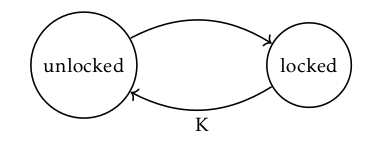
\includegraphics[width=200pt]{img/concurrency/transition-lock}
  \end{figure}
\end{itemize}

\subsubsection{Proofs}
There are 5 proof obligations to ensure that the implementation, predicates and tokens 
\begin{enumerate}
	\item $\text{isLock}(v,P,\gamma)$ is persistent since invariants and equality are persistent and conjunction and existential quantification preserves persistency
  \item $\text{locked}(\gamma)$ is not duplicable since $\Key \cdot \Key = \bot$ and therefore $\dboxed{\Key}^\gamma * \dboxed{\Key}^\gamma \vdash \dboxed{\Key \cdot \Key} ^ \gamma$ by \texttt{OWN-OP} which yields false by \texttt{OWN-VALID} by transitivity of $\vdash$ we are done 
  \item The specification of allocating a new lock is shown by showing the following triple
  \[
    \{P\} \text{newLock}() \{v.\exists \gamma . \text{isLock}(v,P, \gamma)\}
  \]
  by \texttt{HT-BETA} 
  \[
    \{P\} \iref(\false) \{v.\exists \gamma . \text{isLock}(v,P, \gamma)\}
  \]
  a new ghost state is allocated using \texttt{GHOST-ALLOC} and then \texttt{HT-CSQ} together with \texttt{HT-EXIST} and thus we are left with proving
  \[
    \{\text{locked}(\gamma) * P\} \iref(\false) \{v. \exists \gamma. \text{isLock}(v,P,\gamma)\}
  \]
  for some $\gamma$. Then the definition of locked is used
  \begin{equation*}
    \{\dbox{K}^\gamma * P\} \text{ref}(\text{false}) \{v. \exists \gamma. \text{isLock} (v, P, \gamma)\}
  \end{equation*}
  The \texttt{HT-BIND-DET} rule is used with an empty evaluation context. The following 
  \[
    \{\dbox{K} * P\} \text{ref}(\text{false}) \{v.\exists \ell. v= \ell \land \ell \hookrightarrow \text{false} * \dbox{K} * P\}
  \]
  is first proven as follows
  \[
  \begin{prooftree} 
    \infer0[\texttt{HT-ALLOC}]{\{\text{True}\} \text{ref}(\text{false}) \{v.\exists \ell. v= \ell \land \ell \hookrightarrow \text{false}\}}
    \infer1[\texttt{HT-FRAME}]{\{\dbox{K} * P\} \text{ref}(\text{false}) \{v.\exists \ell. v= \ell \land \ell \hookrightarrow \text{false} * \dbox{K} * P\}}
  \end{prooftree}
  \]
  Thus we are left with proving 
  \[
    \{\ell \hookrightarrow \text{false} * \dbox{K} * P\} \ell \{v. \exists \gamma. \text{isLock} (v, P, \gamma)\}
  \]
  where $\exists$I is used to get a concrete $\ell$ and it is proven as follows
  \[
  \begin{prooftree} 
    \infer0[\texttt{HT-RET}]{\{\text{True}\}  \ell \{v.v=\ell \}}
    \infer1[]{{\later(I(\ell, P, \gamma))\}  \ell \{v.\exists \iota . v=\ell \land \boxed{I(\ell, P, \gamma)}^\iota\}}}
    \infer1[\texttt{HT-CSQ}(1)]{{\later(I(\ell, P, \gamma))\}  \ell \{v.\exists \ell, \iota . v=\ell \land \boxed{I(\ell, P, \gamma)}^\iota\}}}
    \infer1[def.]{\{\later(\ell \hookrightarrow \text{false} * \dbox{K} * P \lor \ell\hookrightarrow \text{true})\}  \ell \{v.\exists \ell, \iota . v=\ell \land \boxed{I(\ell, P, \gamma)}^\iota\}}
    \infer1[\texttt{HT-CSQ}(2)]{\{\ell \hookrightarrow \text{false} * \dbox{K} * P\}  \ell \{v.\exists \ell, \iota . v=\ell \land \boxed{I(\ell, P, \gamma)}^\iota\}}
    \infer1[def.]{\{\ell \hookrightarrow \text{false} * \dbox{K} * P\} \ell \{v. \exists \gamma. \text{isLock} (v, P, \gamma)\}}
  \end{prooftree} 
  \]
  In \texttt{HT-CSQ}(1) $\exists$I and $\forall$I can be used to prove that the $\exists$ can be removed in the post condition. For \texttt{HT-CSQ}(2) should be proven 
  \[
    \vdash \ell \hookrightarrow \text{false} * \dbox{K} * P  \Rightarrow \later(\ell \hookrightarrow \text{false} * \dbox{K} * P \lor \ell\hookrightarrow \text{true})
  \]
  which can be proven as follows
  \[
  \begin{prooftree} 
    \infer0[\texttt{Asm.}]{\ell \hookrightarrow \text{false} * \dbox{K} * P  \vdash \ell \hookrightarrow \text{false} * \dbox{K} * P }
    \infer1[$\lor$IL]{\ell \hookrightarrow \text{false} * \dbox{K} * P  \vdash \ell \hookrightarrow \text{false} * \dbox{K} * P \lor \ell\hookrightarrow \text{true}}
    \infer1[$\later$weak]{\ell \hookrightarrow \text{false} * \dbox{K} * P  \vdash \later(\ell \hookrightarrow \text{false} * \dbox{K} * P \lor \ell\hookrightarrow \text{true})}
    \infer1[$\Rightarrow$I]{\vdash \ell \hookrightarrow \text{false} * \dbox{K} * P  \Rightarrow \later(\ell \hookrightarrow \text{false} * \dbox{K} * P \lor \ell\hookrightarrow \text{true})}
  \end{prooftree}
  \]
  \item The specification of the acquire operation is shown by first using the derived rule for recursive functions (from Exercise 6.4) i.e. assuming 
  \[
    \forall v, P, \gamma . \{\later \text{isLock}(v, P, \gamma)\} \text{acquire} \; v \{v.P * \text{locked}(\gamma)\}
  \]
  the following triple 
  \[
    \{\text{isLock}(v,P, \gamma) \} \iif \; \icas (v,\false,\true) \; \ithen \; () \; \ielse \; \text{acquire}(v) \{v.P * \text{locked}(\gamma)\}
  \]
  is shown. Using the $\text{isLock}(v,P,\gamma)$ together with \texttt{HT-PRE-EQ} and moving the invariant into the context we get the following
  \[
    \inv{I(\ell,P,\gamma)^\iota} \vdash \{\True\} \iif \; \icas (v,\false,\true) \; \ithen \; () \; \ielse \; \text{acquire}(\ell) \{v.P * \text{locked}(\gamma)\}
  \]
  then the cas expression is evaluated with the \texttt{HT-BIND} rule by first shown the following triple
  \[
    \inv{I(\ell,P,\gamma)^\iota} \vdash \{\True\} \icas (v,\false,\true) \{v.(u = \true * P * \text{locked}(\gamma) \lor (u = \false))\}
  \]
  since cas is atomic the \texttt{HT-INV-OPEN} rule can be used and thus it suffices to show that
  \begin{align*}
    &\{\later I(\ell, P, \gamma)\} \\
    \inv{I(\ell, P, \gamma)}^\iota \vdash \; & \quad \icas(\ell, \false, \true) \\
    &\{v.(u = \true * P * \text{locked}(\gamma) \lor (u = \false)) * I(\ell, P, \gamma)\}
  \end{align*}
  Then we case on the invariant using the \texttt{HT-DISJ} rule. For the first case
  \begin{align*}
    &\{\later (\ell \hookrightarrow \false * \text{locked} \; \gamma * P)\} \\
    \inv{I(\ell, P, \gamma)}^\iota \vdash \; & \quad \icas(\ell, \false, \true) \\
    &\{v.(u = \true * P * \text{locked}(\gamma) \lor (u = \false)) * I(\ell, P, \gamma)\}
  \end{align*}
  by \texttt{HT-CSQ} it suffices to establish either choice of the disjunctions in the postcondition. The following is chosen
  \[
    u = \true * P * \text{locked}(\gamma) * \ell \hookrightarrow \true 
  \]
  Which follows from using \texttt{HT-FRAME} and \texttt{HT-CAS-SUCC}. \smallskip \\
  In the second case we show
  \begin{align*}
    &\{\later (\ell \hookrightarrow \true)\} \\
    \inv{I(\ell, P, \gamma)}^\iota \vdash \; & \quad \icas(\ell, \false, \true) \\
    &\{v.(u = \true * P * \text{locked}(\gamma) \lor (u = \false)) * I(\ell, P, \gamma)\}
  \end{align*}
  which can be shown by \texttt{HT-CSQ} and establishing the following postcondition
  \[
    u = \false * \ell \hookrightarrow \true 
  \]
  and this follows from the \texttt{HT-CAS-FAIL} rule. \smallskip \\
  Then by the \texttt{HT-BIND} rule the following obligation remains
  \[
    \inv{I(\ell,P,\gamma)}^\iota \vdash \{u = \true * P * \text{locked}(\gamma) \lor u = \false\} \iif \; u \; \ithen \; () \; \ielse \; \text{acquire} \; \ell \{\_.P*\text{locked}(\gamma)\}
  \]
  The two cases in the precondition are considered using the \texttt{HT-DISJ} rule. Then the rules \texttt{HT-IF-TRUE} and \texttt{HT-IF-FALSE} is used on both cases and thus the following two things remains
  \begin{align*}
    &\inv{I(\ell, P, \gamma)^\iota} \vdash \{P * \text{locked}(\gamma)\} () \{\_. P * \text{locked}(\gamma)\} \\
    &\inv{I(\ell, P, \gamma)^\iota} \vdash \{\True\} \text{acquire} \; \ell \{\_. P * \text{locked}(\gamma)\} \\
  \end{align*}
  The first follows by the rule for the unit expressions and the second by the induction hypothesis. 
  \item The specification of the release operation by showing the following triple
  \[
    \{\text{isLock}(v,P, \gamma) * P * \text{locked}(\gamma)\} \text{release} \; v \{\_. \True\}
  \]
  Using the definition of $\text{isLock}(v,P,\gamma)$ the location governed by an invariant can be substituted into the expression under evaluation using the \texttt{HT-PRE-EQ} rule, and by the \texttt{HT-BETA} rule we get the following
  \[
    \{\inv{I(\ell, P, \gamma)}^\iota * \text{locked}(\gamma)\} \ell \leftarrow \false \{\_. \True\}
  \]
  Then the \texttt{HT-INV-OPEN} rule is used by moving the invariant into the assumption (since they are persistent) and thus we get the following triple
  \[
    \inv{I(\ell, P, \gamma)}^\iota \vdash \{\later I(\ell, P, \gamma) * P * \text{locked}(\gamma)\} \ell \leftarrow \false \{\_. \later I(\ell, P, \gamma)\}
  \]
  The two cases in the disjunction in $I(\ell, P, \gamma)$ are considered in the precondition. The first case is 
  \[
    \inv{I(\ell, P, \gamma)}^\iota \vdash \{\later (\ell \hookrightarrow \false * \text{locked}(\gamma) * P) * P * \text{locked}(\gamma)\} \ell \leftarrow \false \{\_. \later I(\ell, P, \gamma)\}
  \]
  which is inconsistent as $\text{locked} * \text{locker} \vdash \False$ and thus it follows by \texttt{HT-LATER-FALSE} \smallskip \\
  For the second case
  \[
    \inv{I(\ell, P, \gamma)}^\iota \vdash \{\later (\ell \pointsto \true) * P * \text{locked}(\gamma)\} \ell \leftarrow \false \{\_. \later I(\ell, P, \gamma)\}
  \]
  and in the postcondition the first disjunct is chosen by \texttt{HT-CSQ} and in the precondition the $\later$\texttt{-LATER} is used to get $\later$ 
  \[
    \inv{I(\ell, P, \gamma)}^\iota \vdash \{\later (\ell \pointsto \true) * \later (P * \text{locked}(\gamma))\} \ell \leftarrow \false \{\_. \later (\ell \pointsto \false) * \later(\text{locked}(\gamma) * P)\}
  \]
  which holds by the \texttt{HT-FRAME} and \texttt{HT-STORE}
\end{enumerate}

% \subsection{Bags}
% TODO?

\newpage
%%% Local Variables:
%%% mode: latex
%%% TeX-master: "pav-noter"
%%% End:
